\documentclass[a4paper]{report}
\setlength{\textwidth}{13cm}
\usepackage{amsmath}
\usepackage{amssymb}
\usepackage[ngerman,german]{babel}
\usepackage[utf8]{inputenc}
\usepackage[T1]{fontenc}
\usepackage{graphicx}
\usepackage{listings}
\usepackage{color}
\usepackage{tikz}
\usepackage{pgfplots}
\usepackage{float}
\usepackage{pdfpages}

\author{Marius Unsel}
\title{Positionsregelung mit AVR/Arduino und Python}
\date{\today}
\begin{document}
\maketitle
\tableofcontents
\chapter{Vorwort}
In den folgenden Kapiteln werde ich meinen Fortschritt bei
dem Entwurf einer Positionsregelung dokumentieren.
Die Umsetzung soll mit dem Opensource Mikrocontrollersystem
Arduino stattfinden. Für Debugzwecke, zur Parametrierung des
Reglers und zum Anzeigen der Messergebnisse am Computer dient die serielle Schnittstelle, die zur Daten\"ubertragung zum Computer benutzt wird. Der $\mu$C ATmega2560, der auf dem Arduino Mega verbaut ist wird in C mit Hilfe von der Arduino IDE zur Verf\"ugung gestellten Bibliotheken programmiert. Viele Einstellungen im Mikrocontroller erfolgen über Wertzuweisungen in Register, die sogenannten "'special function register"'. Die notwendigen Werte und Registerbezeichnungen, sowie Codebeispiele zur Anwendung finden sich im Datenblatt des Microcontrollers.

Die seriellen Daten vom Arduino sollen von einem Python-Programm ausgewertet werden. Dieses stellt eine Visualisierung der Messdaten in Echtzeit zur Verf\"ugung und stellt ein Interface bereit, mit dem sich Einstellungen der Regelung bequem per GUI(Graphical User Interface) vornehmen lassen. Die Umsetzung dieses AuswertProgramms wird mit dem GUI-Framework "'Qt"' von Nokia und der Plotbibliothek "'PyQtGraph"' erfolgen. N\"aheres dazu im Kapitel "'Python Interface"'
\\
\\
Hiermit m\"ochte ich meinem Professor Roustaim Chakirov danken, da dieser mir die Freir\"aume gelassen hat, in diesem Semster Dinge zu lernen, die ich mir gr\"{\ss}tenteils selbst ausgesucht habe. Dazu geh\"oren die Grundlagen von Linux, Python und weiterf\"uhrende Kenntnisse \"uber Atmel Mikrocontroller sowie die absoluten Grundlagen des Satzsystems LATEX.

\chapter{Aufbau}
\begin{figure}[h]
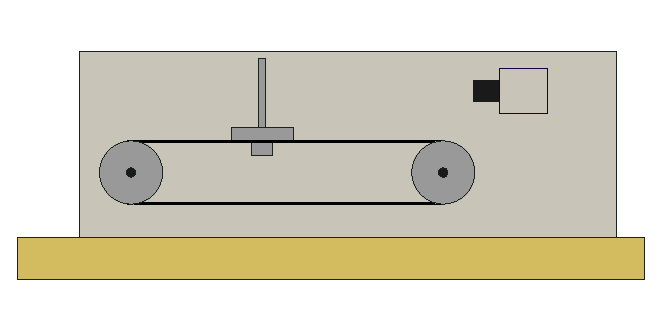
\includegraphics[width=\textwidth]{img/position_control_sheme.pdf}
\caption{Skizze des Modells}
\end{figure}
Die Regelstrecke besteht aus einem Keilriemen, der zwischen zwei Umlenkrollen gespannt ist. Der Riemen wird von einem DC-Motor an einer der Rollen angetrieben und treibt einen Schlitten, der auf einer Linearf\"uhrung sitzt an. An diesem Schlitten ist eine Metallplatte befestigt, mit dessen Hilfe der Sensor den Abstand des Schlittens zum Sensor bestimmen kann. Die Metallplatte reflektiert dabei die Infrarotstrahlung, die vom Sensor ausgestrahlt wird.
\subsection{Bauteile}
\begin{itemize}
\item 12V DC Motor
\item SHARP Sensor
\item Avago Inkrementalgeber
\item Arduino Mega2560
\item DFRobot Moto Shield
\item igus Linearf\"uhrung und Schlitten
\item Keilriemen
\item zwei Umlenkrollen
\item Grundplatte mit Spannvorrichtung
\end{itemize}
\subsection{Blockschaltbild}



\chapter{SHARP low-cost Distanzsensor auswerten}
Der in diesem Versuch verwendete Infrarot-Distanzsensor von SHARP liefert eine analoge Spannung, die umgerechnet werden kann in die entsprechende Distanz. Da diese Kennlinie nicht linear ist und die entsprechende Funktion nicht bekannt ist, wird ein Verfahren zur linearen Interpolation verwendet, um aus einem Messwert und zwei Vektoren mit bekannten x-, sowie y-Koordinaten die entsprechende Distanz anzun\"ahern.

\section{Kennlinie des Sensors}
\begin{figure}[H]
\includegraphics[width=\textwidth]{img/kennlinie.pdf}
\caption{Kennline $x(u)$}
\end{figure}
Die Kennlinie des Sensors wurde mit Hilfe eines Multimeters und einem Maßband Gemessen. Der Abstand zwischen zwei Messungen betr\"agt 10mm.
\section{Lookuptable mit linearer Interpolation}
Die Spannungswerte $U_1, U_2, ..., U_n$  des Sensors in der Einheit Volt lauten:\\ \\
\([0.51, 0.57, 0.61, 0.65, 0.69, 0.73, 0.77, 0.83, 0.9, 0.96, 1.05, 1.15, 1.28, 1.42, 1.61, 1.85, 2.15, 2.54]\)\\ \\
Diese sind in aufsteigender Gr\"osse sortiert, damit der Algorithmus richtig funktioniert. f\"ur die entsprechenden Diszanzwerte $x_1, x_2, ..., x_n$  in der Einheit Millimeter gilt diese Sortierung nicht, da jeder Wert $x_i$ von einem entsprechenden Wert $U_i$ abh\"angt. Die Distanzwerte lauten:\\ \\
\([240, 220, 200, 180, 170, 160, 150, 140,130, 120, 110, 100, 90, 80, 70, 60, 50, 40] \)
\begin{figure}[H]
\centering
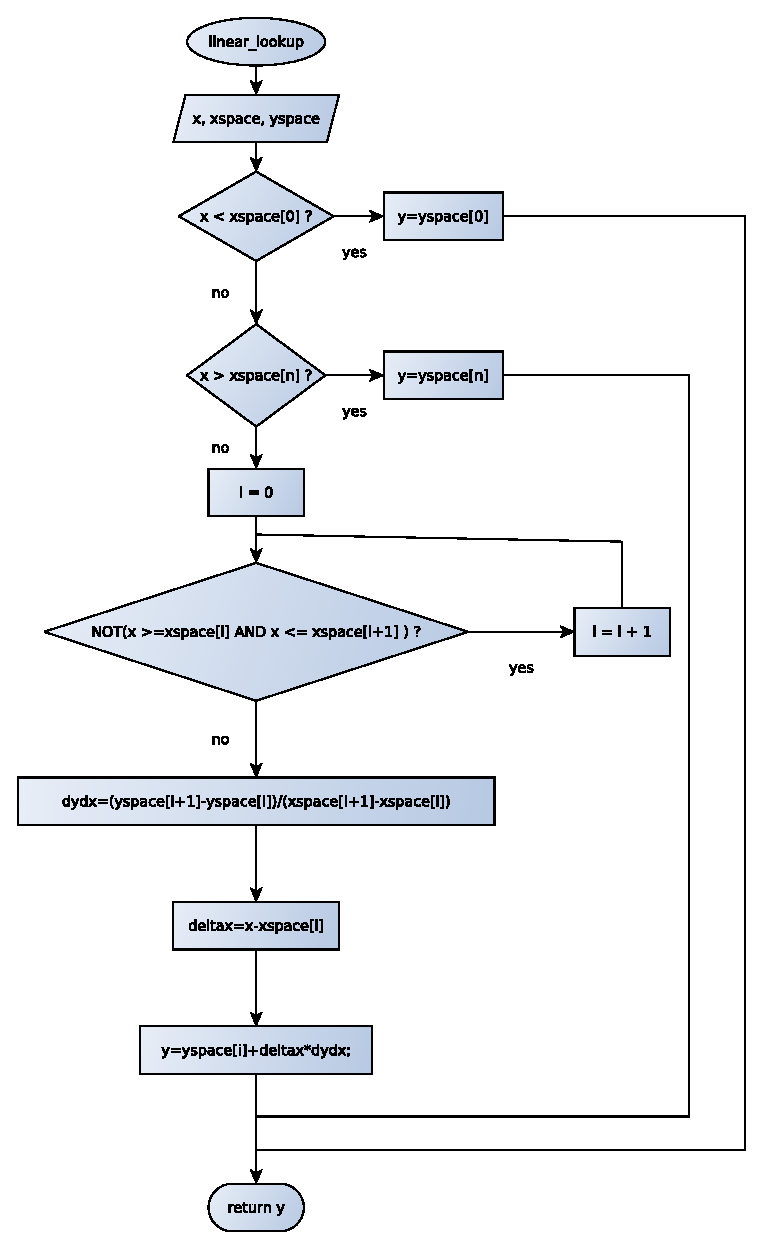
\includegraphics{img/lookup_diagram.pdf}
\caption{Algorithmus einer linearen Interpolation}
\end{figure}
 Die Interpolationsroutine pr\"uft zuerst, ob, und zwischen welchen Spannungswerten die gemessene Spannung liegt. Liegt die Spannung ausserhalb, so wird das entsprechende Randelement aus der Distanztabelle($x_1$ oder $x_n$) ausgegeben. Eine Extrapolation findet nicht statt. Liegt der Wert $U_{mess}$ nun zwischen $U_i$ und $U_{i+1}$, so wird der Differenzenquotient $\frac{\Delta x}{\Delta U}=\frac{x_{i+1}-x_i}{U_{i+1}-U_i}$  und der Abstand zwischen $U_{mess}$ sowie $U_i$ gebildet. Der interpolierte Distantwert ergibt sich dann durch $x=U_i+\frac{\Delta x}{\Delta U}*(U_{mess}-U_i)$. Die Abbildung 3.2 zeigt das Flussdiagramm des implementierten Algorithmus.

\chapter{Avago Drehencoder auslesen}
Beim Drehencoder von Avago handelt es sich um einen optischen 3-Kanal Encoder. F\"ur dessen Auswertung wurde eine Interrupt Rooutine so eingestellt, dass diese jedes mal, wenn auf dem ersten Kanal eine positive Flanke erkannt wird aufgerufen wird. In dieser Routine wird dann gep\"uft, ob der aktuelle Digitalwert auf dem zweiten Kanal HIGH oder LOW ist und dementsprechend wird eine Z\"ahlervarible hoch, bzw runter gez\"ahlt. Aus diesem Z\"ahlerstand kann in regelm\"a{\ss}igen Abst\"anden durch den Regleralgorithmus eine Umrechnung in eine entsprechende Winkelgeschwindigkeit, einen Winkel oder die entsprechende Position des Schlittens erfolgen. Der Encoder liefert pro Kanal 500 Impulse, es werden pro Umdrehung also 500 positive Flanken von Kanal A ausgewertet.
\begin{figure}[H]
\includegraphics[width=\textwidth]{img/encoder_channels.pdf}
\caption{Kanal A und B des Encoders}
\end{figure}

\chapter{Regler-Algoritmus}
\section{Beschreibung der Funktionsweise}
Der Regler auf dem AtMega2560 ist als diskreter PID Regler realisiert. Dieser nimmt eine Struktur aus Zustandsvariablen und Reglerparametern entgegen und berechnet daraus die Stellgröße. Außerdem lässt sich durch Senden von Befehlen \"uber die serielle Schnittstelle einstellen, welchen Zustand(Position oder Geschwindigkeit) als Grundlage f\"ur den Algorithmus verwendet wird.
Eine neue Stellgr\"osse wird 100 mal pro sekunde berechnet. Der Kehrwert von 10ms fliesst als Konstante mit in die Berechnung ein, damit die Zust\"ande in den Einheiten Sekunde und Millimeter abgespeichert sind. Die Zeitparameter $\frac{1}{T_a}$ und $T_v$ sind dann ebenfalls in der Einheit $\frac{1}{s}$ bzw. $[s]$ und der Verst\"arkungsfaktor $[K_p]=[\frac{1}{mm}]$. Somit lassen sich die gleichen Parameter, wie aus dem Simulink Modell in dieser Regelung \"ubernhemen. \\
Die Standardabweichung ist: \[e(t)=w(t)-x(t)\] Dabei ist $x$ der Istwert und $w$ die F\"uhrungsgr\"o{\ss}e. Die Formel eines PID-Reglers ist: \[y(t)=K_p\left(e(t)+\frac{1}{T_a}*\int_0^t e(t) \,dt +T_v*\frac{de}{dt}\right)\]
Da wir allerdings nur in festgelegten Abst\"anden $T=10ms=0,01s$ eine neue Stellgr\"osse berechnen k\"onnen, m\"ussen die kontinuierlichen Anteile $\int_0^t e(t) dt$ und $\frac{de(t)}{dt}$ der Gleichung durch diskret berechenbare Formelteile ersetzt werden. Das Integral l\"asst sich numerisch durch eine Summe ann\"ahern:
\[\int_0^t e(t) \,dt \approx \sum e(kT)*T \qquad\mbox{f\"ur} \qquad k \in \mathbb{N}\]
Die Ableitung der Standardabweichung  l\"asst sich auch als Differenzenquotient darstellen. Man wechselt dabei von der Tangentensteigung zu einer Sekantensteigung:
\[\frac{de(t)}{dt} \approx \frac{e(kT)-e((k-1)T)}{T} \]

Somit ergibt sich die Reglergleichung:
\[ y(kT)=K_p\left(e(kT)+\frac{T}{T_a}*\sum e(kT)  +T_v*\frac{e(kT)-e((k-1)T)}{T}\right)\]
Damit der integrierende Anteil der Gleichung nicht ins Unermessliche anwachsen kann, wird dieser ab einem bestimmten Wert festgelegt. Diese Grenze l\"asst sich durch ausprobieren ermitteln.
\section{Bestromung des Motors mit H-Br\"ucke}
Das Motoshield ist in der Lage, zwei Gleichstrommotoren in beide Drehrichtungen zu treiben. Es enth\"alt als zwei H-Br\"ucken. Da wir nur einen Motor in unserer Regelung verwenden, ben\"otigen wir nur eine dieser Br\"ucken. F\"ur die Ansteuerung eines Motors ben\"otigt man zwei Ausg\"ange des Arduino. Einen zur Drehrichtungsbestimmung und einen zur Steuerung der gemittelten Spannung durch eine PWM. Liegt auf dem Richtungsausgang ein HIGH-Pegel an, so dreht sich der Motor die eine Rihtung, liegt ein LOW-Pegel an, so dreht er sich anders herum. Die PWM wurde durch Registerbefehle des AtMega2560 so ver\"andert, dass Sie mit einer Tr\"agerfrequenz von $\approx 31kHz$ arbeitet, sodass die Ansteuerung des Motors nicht mehr f\"r das menschliche Auge h\"orbar ist. Dessen Duty-Cycle hat eine Aufl\"osung von 8bit, also  lassen sich mit dem Arduino-Befehl \tt analogWrite(PWM-pin,Wert) \rm die Werte $0...255$ verarbeiten. Also muss durch die Routine der Motorbestomung sichergestellt werden, dass der Stellgrad bei negativem Wert die H-Br\"ucke anders bestromt als bei positivem Wert und dessen Betrag bei $255$ begrenzt wird.

\section{Anmerkung zur praktischen Umsetzung}
Der Regleralgorithmus wurde komplett mit Flie{\ss}kommazahlen berechnet. Das liegt daran, dass das rapid-prototyping-Simulink-Modell ebenfalls mit floats rechnet und  die Lookuptable mit floats rechnet. Dies ist auf einer kleinen Maschine wie einem Mikrocontroller keine praxistaugliche L\"osung, da dessen Ressourcen stark begrenzt sind und die Berechnung einer neuen Stellgr\"o{\ss}e mit diesem Datentyp viel zu lange dauert. Au{\ss}erdem sind die Messdaten des Infrarotsensors und des Drehencoders, sowie dem Stellwert der H-Br\"ucke integer-Werte. Somit w\"are es wesentlich effizienter, die Berechnung des Stellgrades ebenfalls mit integer-Werten durch zu f\"uhren. Da der Versuchsaufbau nichts anderes macht, als zu regeln, l\"asst sich dennoch eine Frequenz von $100Hz$ erreichen, was f\"ur diese tr\"age mechanische Regelstrecke ausreicht. Ist die Regelung allerdings Teil eines komplexeren Systems, muss eine effizientere Methode verwendet werden. Eine Methode w\"are, die obere Reglergleichung zu vereinfachen:
\[ y(kT)=K_p\left(e(kT)+\frac{1}{T_a}*\sum e(kT)  +T_v*(e(kT)-e((k-1)T)\right)\]
Au{\ss}erdem ist es auch nicht n\"otig, im Mikrocontrollerprogramm mit korrekten Einheiten zu arbeiten. Man rechnet einfach mit den direkt aufgenommenen Messdaten, statt eine Umwandlung vor zu nehmen. M\"ochte man dann einen Sollwert in einer Einheit wie z.B. $\frac{mm}{s}$ einstellen, so muss man au{\ss}erhalb des Programms eine Umrechnung durchf\"uhren und dem Mikrocontroller diesen Wert mitteilen.
\section{Simulink-Modell}
Dem folgenden Simulink-Modell ist das C-Programm nachempfunden. Die dort ermittelten Reglerparameter funktionieren genau so im selbst geschriebenen Programm.
\includepdf{img/simulinkmodell.pdf}
\chapter{Python Interface}
\section{Warum Python?}
Um den Regler bequem einstellen zu k\"onnen sowie die Messdaten in Echtzeit in einem Graphen dar zu stellen, wird ein kleines Python-Proramm erstellt, dass als Interface für den regler dienen soll. Die Wahl fiel auf Python, da sie eine sehr leicht zu erlernende Programmiersprache ist und nichts kostet, da Open Source. Somit lassen sich auf einem System geschriebene Programme auf vielen Sytemen laufen, ohne Lizenzgebühren f\"ur einen Interpreter oder eine Runtime-Umgebung f\"ur jedes System neu zu kaufen. Die Anwendung soll sowohl auf einem PC, als auch auf einem eingebetteten System, wie dem Raspberry Pi oder dem Beaglebone laufen. Außerdem gibt es mit den Erweiterungen "'Numpy"', "'Scipy"' und "'Matplotlib"' sehr m\"achtige numerische sowie wissenschaftliche Funktionen, die die h\"aufigsten MATLAB-Funktionen abdecken und von dessen Syntax her nahezu identisch sind. 
\section{Oberfl\"ache}
Die Grafische Oberfl\"ache des Interfaces wurde mit dem Qt Designer erstellt. Mit diesem freien Editor lassen sich GUIs nach dem Prinzip WYSIWYG(what you see is what you get) erstellen. Er ist bei der Installation des Qt Frameworks mit enthalten. Da es sich bei Qt eigentlich um ein C++ Framework handelt, muss die mit dem Designer erstellte *.ui-Datei mit Hilfe eines \"Ubersetzers in ein Python Skript konvertiert werden. Das \"Ubersetzerprogramm heißt "'pyuic4"' und erstellt ein Skript mit einer Window-Klasse, die recht einfach in ein Hauptprogramm eingebunden werden kann. Neben dem Python-Interpreter sind folgende Zusatzbibliotheken n\"otig:
\begin{itemize}
\item PyQt4
\item PySerial
\item PyQtGraph
\item numpy
\item scipy und matplotlib(optional)

\end{itemize}
\section{Serielle Kommunikation}
F\"ur die Kommunikation \"uber die serielle Schnittstelle mit dem Arduino wird die "'Serial"'-Bibliothek verwendet. Au{\ss}erdem kommt die "'Threading"'-Bibliothek zum Einsatz, mit der in einem seperaten Thread permanent den Eingang der Schnittstelle abgefragt wird und ein Buffer dementsprchend gef\"ullt wird. Dieser Buffer wird in regelm\"a{\ss}igen Abst\"anden ausgelesen, geleert und dessen Inhalt in einem Array gespeichert, dass als Grundlage f\"ur den live-Plot dient.
\begin{figure}[h]
\includegraphics[width=\textwidth]{img/interfacewindow.png}
\caption{Aussehen des Interfaces}
\end{figure}
Die serielle Kommunikation sollte mit Zeitstempel und folgendem 16 bit Integer-Wert vom Mokrocontroller zum Python-Interface erfolgen. Au{\ss}erdem soll vom Interface einzelne character zur Erkennung mit folgenem Eintsellwert als Integer zum Microcontroller gesendet werden, um Einstellungen der Ausgabe oder der Parameter durch das Interface vorgenommen werden k\"onnen. Diese Schritte sind aus Mangel an Zeit und fehlender Erfahrung im Umgang mit dem Signal-Slot-System, mit dem sich Events mit GUI-Elementen verkn\"upfen lassen nicht implementiert. Eine einfache Plotanwendung, die Strings gefolgt von einem \tt linefeed \rm als \tt float \rm  interpretiert und plottet funktioniert hingegen und liegt den Anlagen ebenfalls bei.
\chapter{Quellen}
\begin{itemize}
\item www.arduino.cc
\item http://www.rn-wissen.de/index.php/Regelungstechnik
\item PyQt und PySide - Peter Bouda ISBN 978-3-941841-50-5
\item http://www.mikrocontroller.net/articles/AVR-GCC-Tutorial
\item Datenblatt des Atmega2560
\item MATLAB/Simulink Hilfe
\end{itemize}	  
\end{document}
